% use UTF-8 encoding in editors such as TeXworks
% !TEX encoding = UTF-8 Unicode
% !TEX TS-program = pdflatex

\documentclass[%
    corpo=13.5pt,
    twoside,
%    stile=classica,
    oldstyle,
%    autoretitolo,
    tipotesi=magistrale,
    greek,
    evenboxes
]{toptesi}

\usepackage[utf8]{inputenc}% codifica d'entrata
\usepackage[T1]{fontenc}%    codifica dei font
\usepackage{lmodern}%        scelta dei font
\usepackage{listings}       % code listing

% Vedere la documentazione toptesi-it.pdf per le
% attenzioni che bisogna usare al fine di ottenere un file
% veramente conforme alle norme per l'archiviabilità.

\usepackage{hyperref}
\hypersetup{%
    pdfpagemode={UseOutlines},
    bookmarksopen,
    pdfstartview={FitH},
    colorlinks,
    linkcolor={blue},
    citecolor={blue},
    urlcolor={blue}
  }

%%%%%%% Definizioni locali
\newtheorem{osservazione}{Osservazione}% Standard LaTeX
\ExtendCaptions{english}{Abstract}{Acknowledgements}



\begin{document}\errorcontextlines=9

% set english ad primary language
\english

%%%%%%%%%%%%%%%%%%%%
% BEGIN front page %
%%%%%%%%%%%%%%%%%%%%
\begin{ThesisTitlePage}*

\ateneo{Politecnico di Torino}
\nomeateneo{DEPARTMENT OF CONTROL AND COMPUTER ENGINEERING}
\CorsoDiLaureaIn{Master of Science in}
\corsodilaurea{Computer Engineering}
\TesiDiLaurea{Master Degree Thesis}

\titolo{Deep Learning on Polito Knowledge Graph}
\sottotitolo{Leveraging Relational GCN for link prediction between nodes of a newly built publications graph}

\CandidateName{Candidate}
\candidato{Giovanni \textsc{Garifo}}

\AdvisorName{Supervisors}
\relatore{Prof.~Antonio Vetrò}
\secondorelatore{Prof.~Juan Carlos De Martin}
\sedutadilaurea{\textsc{Academic~Year} 2018-2019}%

\logosede[6cm]{logopolito}
\end{ThesisTitlePage}
%%%%%%%%%%%%%%%%%%
% END front page %
%%%%%%%%%%%%%%%%%%


% offset rilegatura
%\setbindingcorrection{3mm}

\makeatletter
\newenvironment{miadedica}{
    \clearpage
    \if@twoside
        \ifodd\c@page\else\thispagestyle{empty}\null\clearpage\fi
    \fi
    \thispagestyle{empty}%
    \list{}{\labelwidth\z@
    \leftmargin.73\textwidth
    \parindent\z@
    \raggedright\LARGE\itshape}\item[]
    \normalsize
}

\begin{miadedica}
    To Monia\\
    To my Grandfather
\end{miadedica}


\paginavuota
\sommario

Summary here, one page


\ringraziamenti

Acknowledgements here, half page


\tablespagetrue\figurespagetrue % normalmente questa riga non serve ed e' commentata
\indici

\mainmatter

\chapter{Introduction}

\section{Motivation}

Graphs are used to empower some of the most complex IT services available
today. They can be used to represent almost any kind of information, and
they are particurlarly capable of representing the structure of complex
system, thus to express the relations between its elements.
\newline
\newline
In the past ten years, a lot of effort has been put into trying to leverage the power
of graphs to represent human knowledge and to build search tools capable of
query and understand the semantic relations inside such graphs. RDF graphs are a
particular class of graphs that can be used to build knowledge
repositories. Given a domain and an ontology, they allows to build a structured
representaion of the knowledge of such domain.
\newline
\newline
Modern machine learning techniques can be used to mine latent informations
from such graphs. One of the main challenges in this field is how to learn
meaningful representations of the graph nodes that embed the underlying
knowledge. Such representations can be then used to evaluate new
links inside the graph, task commonly known as link prediction, or to classify
unseen nodes. Deep learning techniques have proved to be first class citizens when
dealing with representation learning tasks, being able to learn the latent
representation of nodes without any prior knowledge other than the graph structure,
so as not to require any feature engineering.



\section{Thesis structure}

\subsection{Chapter 2}

\subsection{Chapter 3}

\subsection{Chapter 4}



\chapter{Background}

\section{Semantic Web}

\subsection{From a Web of content to a Web of data}

The World Wide Web has been developed as a tool to easily access documents
and to navigate through them by following hyperlinks. This simple description
already resembles the structure of a graph: we can think of documents as
nodes, and of hyperlinks as edges. The unstoppable growth of the "web graph" led to
the emergence of new tools to extricate in such complexity. Search engines have been
developed to easily navigate such a giant graph, by scoring search results based on
trivial statistics, such as the number of times a document has been linked.
\newline

The Web rapidly became one of the most disruptive technology ever built, but it's power
was limited to the fact that it was exploitable only by human beings. To build a more
comprehensive system, where informations can be not only machine-readable, but
machine-understandable, thus to allow new usage of such a giant source of informations,
the WWW had to move from a web of content, to a web of data.
\newline

The World Wide Web Consortium (W3C) introduced the Semantic Web as an extention
to the prior standard of the WWW. It's primary goal has been
to define a framework to describe and query semantic informations contained
in the documents available on the web, so as to allow machines to understand
the semantic informations contained in web pages. In the vision of Tim
Berners-Lee, the father of WWW, this will bring to the transition from a
World Wide Web to a Giant Global Graph, the GGG, where a
web page contains metadata that provides to a machine the needed information to
understand the concepts and meanings expressed in it.



\subsection{The Semantic Web building blocks}

The three key components of the Semantic Web standards are:
\begin{enumerate}
\item OWL: the Web Ontology Language
\item RDF: the Resource Description Framework
\item SPARQL: The SPARQL Protocol and RDF Query Language
\end{enumerate}
\bigskip

OWL is a language used to define ontologies. In this context, an ontology
is defined as a collection of concepts, relations and constraints between
these concepts that allows to describe an area of interest or a domain.
OWL allows to classify things in terms of their meaning by describing
their belonging to classes and subclasses defined by the ontology: if
a thing is defined as member of a class, this means that it shares the
same semantic meaning as all the other members of such class. The result of
such classification is a taxonomy that defines a hierarchy of how things
are semantically interrelated in the domain under analysis.
The instances of OWL classes are called individuals, and can be related
with other individuals or classes by means of properties. Each individual
can be characterized with additional informations using literals, that
represent data values like strings, dates or integers.
\newline

RDF is a XML-based framework that defines a standard model for the
description, modelling and interchange of resources on the Web.

The first component of the framework is the "RDF Model and Syntax",
which defines a data model that describes how the RDF resources should be
represented. The basic model consist of only three object types: resource,
property, and statement.
A resource is uniquely identified by an Uniform Resource Identifier (URI).
A property can be both a resource attribute or a relation between resources.
A statement describes a resource property, and is defined as a triple
between a subject (the resource), a predicate (the property) and an
object (a literal or another resource).

The second component of the framework is the "RDF Schema" (RDFS),
that defines a basic vocabulary for describing RDF resources and the
relationships between them. Many vocabularies have been built on top of
RDFS, such as the Friend of a Friend (FOAF) vocabulary, for describing
social networks, or the one maintained by the Dublin Core Metadata
Initiative, that defines common terms used in the definition of metadata
for digital resources.

\begin{figure}[ht]
\centering
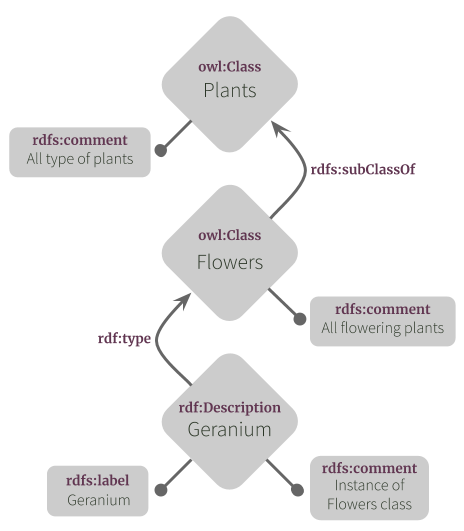
\includegraphics[scale=0.6]{img/owl-ontology-example.png}
\caption{An example of ontology defined using OWL and RDF Schema.}
\label{fig:owl-ontology-example} %used with \ref{imglabel}
\end{figure}

SPARQL is a query language for triplestores, a class of Database
Management Systems (DBMS) specialized in storing RDF databases. Such DBMS
often expose endpoints that can be used to query the database and obtain
results. Given the complexity of the data stored, the query language has
been designed to be as simple as possible, in example by allowing the use
of variables, whose definition is preceded by a question mark.

The syntax of SPARQL is heavily derived from SQL, with some
minor adaptations to be more suited for querying graphs data. The
following is an example of query which select all the labels
(human-readable description of a resource) of all the entities that
matches the given resource type.

\begin{lstlisting}[
        language=sparql,
        frame=single,
    ]
    PREXIF plants:<http://example.org/plants/>

    SELECT ?name
    WHERE {
        ?subject rdf:type plants:flowers .
        ?subject rdfs:label ?name .
    }
\end{lstlisting}

\subsection{Knowledge Bases as knowledge repositories}

Even if the raise of the Semantic Web has suffered a stunting in its growth
due to the complexity of it's vision, many new project empowered by it's
enabling technologies have arise. Efforts have been put by profit and
non-profit organizations in trying to build complex knowledge repositories
starting from the knowledge already present in the Web. An example among all
is the DBpedia project, which developed a structured knowledge base from the
unstructured data available on Wikipedia. Another example is the so called
"Knowledge Graph" made by Google, which is used to enhance it's search engine
and virtual assistant capabilities, allowing to retrieve punctual informations
about everything that has been classified in it's ontology and described
in it's knowledge base.

From an implementation perspective, knowledge bases can be created to
describe a specific domain by defining an ontology and a vocabulary for
such domain using OWL and RDF Schema, and then by describing the concepts
of such domain using the RDF Model and Syntax. The RDF document can then be
stored in a triplestore that can be queryed using SPARQL. The biggest effort
when building knowledge bases is to have a correctly understanding and prior
knowledge of the domain of interest, to avoid the risk of mischaracterizing
and misrepresenting concepts.

If all the requirements and cautions are met, a well formed knowledge base may
prove to be a critical resource for an organization. It allows not only to
build new services upon it, but also to improve the existing knowledge inside the
company by performing reasoning upon the available knowledge, thus
to discover implicit facts that can be derived from existing relationships.
Another field of applications is the development of Expertise Systems, AI software
that emulates the behaviour of a human decision-making process by
navigating the knowledge base and taking decisions like in a rule-based system.


\begin{figure}[h]
\centering
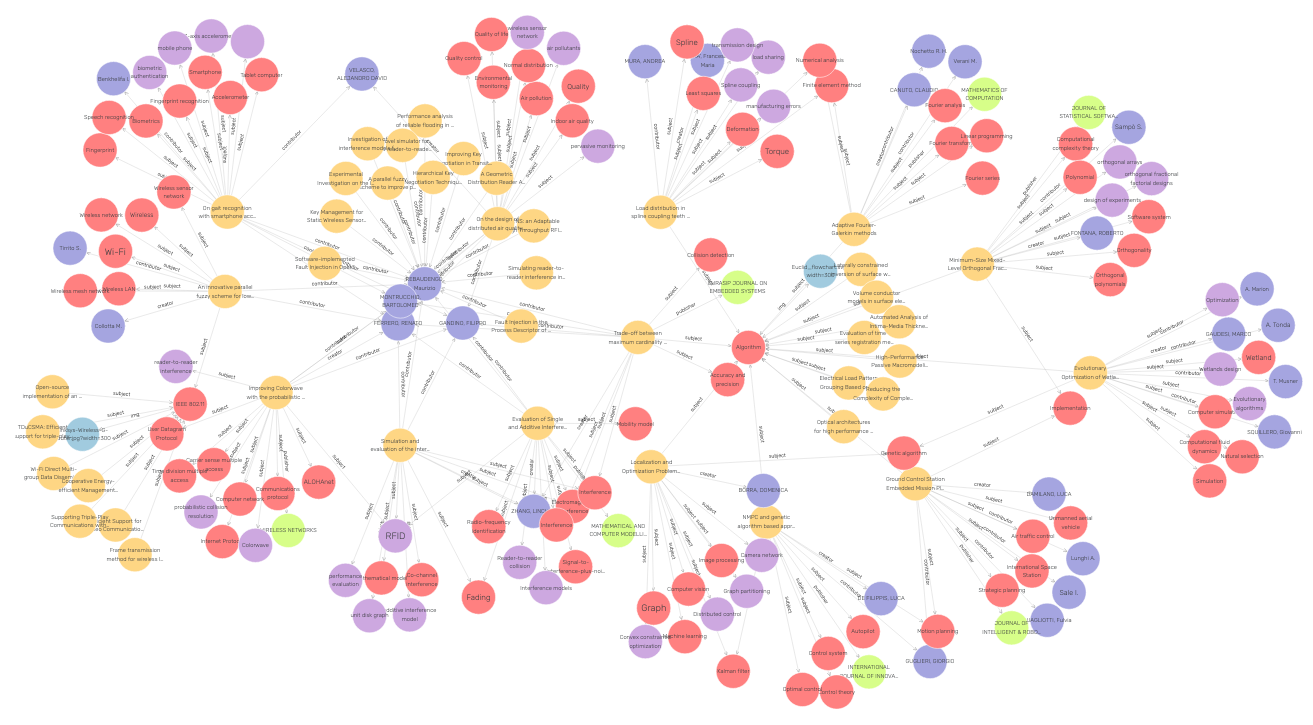
\includegraphics[scale=0.4]{img/geranium-knowledge-base-example.png}
\caption{An extract of the Polito Knowledge Graph.}
\label{fig:geranium-knowledge-base-example} %used with \ref{imglabel}
\end{figure}


In a Big Data era, knowledge bases can't be any less. The vastity of human
knowledge is reflected onto the complexity of the graphs
builded from it. Today's knowledge bases are commonly composed by tens of
thousands nodes and by hundreds of thousands of edges, such giant data
structures pose many challenges.
Not only storing and querying giant graphs requires the adoption
specialized DBMS that are capable of efficiently store and query the RDF
input representation, but also doing analysis and gathering statistics from
such giant graphs requires the adoption of highly efficient algorithms in
order to retrieve the desired output in an acceptable time.

The availability of such a complex and informative data structure leads
to the opening of interesting scenarios, especially when thinking about
the latent informations that can be extracted from it. In
fact, a knowledge base is a structured representation of the
human knowledge in a specific field, thus it's completess is restricted
by the human understanding.


\section{Learning on graphs}

\subsection{representation learning: embeddings}

\subsection{tecniche di ML sui grafi per node embeddings}


\chapter{State of the art}

\chapter{Approach and Methodology}

\chapter{Development and Implementation}

\chapter{Evaluation}

\chapter{Conclusions}


%%%%%%%%%%%%%%%%%%%%%%
% BEGIN bibliography %
%%%%%%%%%%%%%%%%%%%%%%
\begin{thebibliography}{9}
\bibitem{gal} G.~Galilei, {\em Nuovi studii sugli astri medicei}, Manuzio,
        Venetia, 1612.
\bibitem{tor1} E.~Torricelli, in ``La pressione barometrica'', {\em Strumenti
        Moderni}, Il Porcellino, Firenze, 1606.
\bibitem{tor2} E.~Torricelli e A.~Vasari, in ``Delle misure'', {\em Atti Nuovo
        Cimento}, vol.~III, n.~2 (feb. 1607), p.~27--31.
\bibitem{duane1964} Duane J.T., \emph{Learning Curve Approach To Reliability
		Monitoring}, IEEE Transactions on Aerospace, Vol. 2, pp. 563-566, 1964
\end{thebibliography}


\end{document}